\section{Experimental System}

Two separate experimental systems were used when testing and gathering results for localization and motion planning. The first of these is the physical robot, HARLIE, which will be described in further detail in \autoref{subsec:harlie_setup}. The second experimental system is a simulation environment which will be described in detail in \autoref{subsec:simulation_setup}.

\subsection{HARLIE}\label{subsec:harlie_setup}

\begin{figure}
\centering
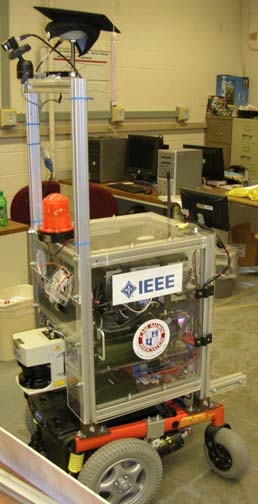
\includegraphics[height=0.5\textheight]{images/harlie}
\caption{HARLIE, the robot used for experimental testing \label{fig:harlie}}
\end{figure}

The physical robot used for these experiments was HARLIE (see \autoref{fig:harlie}). HARLIE is a fully autonomous robot built on top of a wheelchair base donated by the Invacare Corportation. The robot is powered via a pair of car batteries in series, providing a nominal twenty-four volts to the system. The wheelchair base has two electric motors powering the two drive wheels; with one motor per wheel, HARLIE is able to vary the velocity of each drive wheel independently. Because of this independent velocity control, HARLIE can move forwards and backwards, both straight and in arcs, as well as spin in place. This drive setup is known as ``differential drive'' and is one of the most common drive setups used in mobile robotics \autocite{Lav06}.

On top of this differential drive base, HARLIE is equipped with numerous sensors and computing systems. HARLIE is equipped with three sensors that are used for indoor localization: quadrature encoders, a MEMS gyroscope and a LIDAR. The quadrature encoders on HARLIE are used to measure the speed of each of HARLIE's drive wheels; these speeds are then integrated over time to get an estimate of the total distance moved by each wheel. HARLIE also has encoders attached to the two drive shafts, though these are used in the velocity control loops and not for localization. The encoders used on HARLIE (see \autoref{fig:grayhill_encoder}) are high resolution optical encoders, providing over 1000 encoder ticks per wheel revolution (or approximately 58 $\mu$m per tick), which allows for precise measurement of the wheel's speed and direction. The encoders are not directly connected to the wheel's axle - they are connected via a pair of pulleys \todo{is this what those white gear thingies are called?} and a rubber, toothed belt (see \autoref{fig:wheel_encoder_setup}).

\begin{figure}
\centering
\subfloat[Grayhill 61K Optical Encoder]{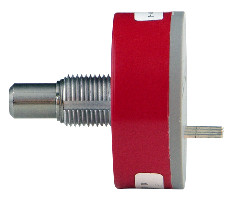
\includegraphics[width=0.5\textwidth]{images/grayhill_encoder}\label{fig:grayhill_encoder}}
\hfill
\subfloat[Wheel Encoder Setup]{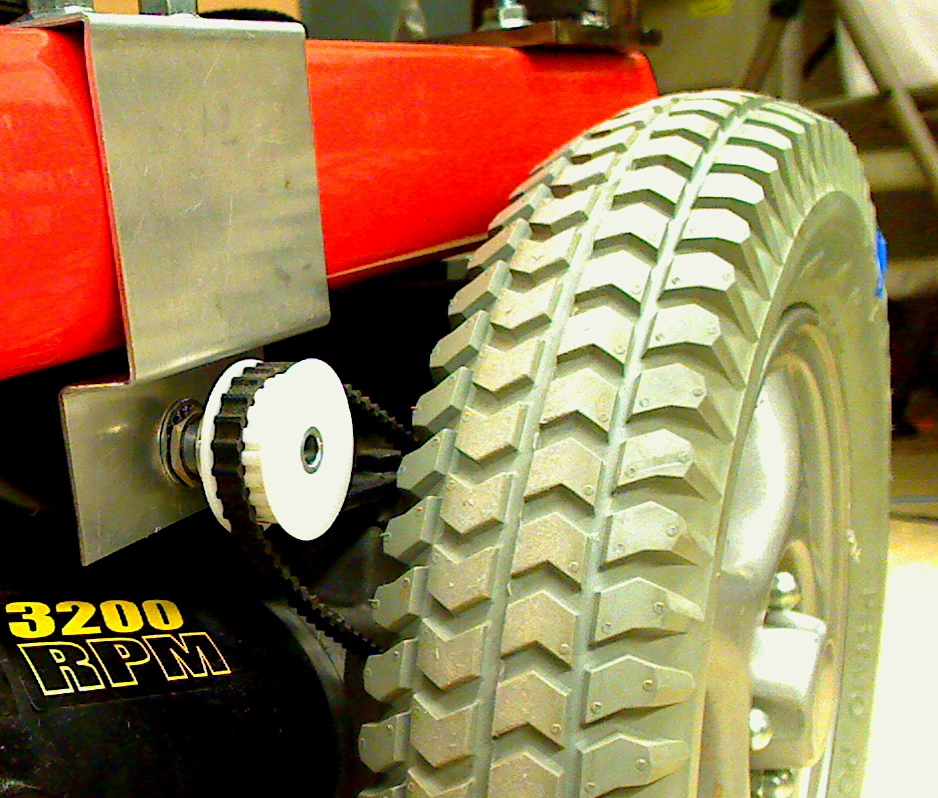
\includegraphics[width=0.5\textwidth]{images/wheel_encoder_setup}\label{fig:wheel_encoder_setup}}
\caption{Encoder \& Encoder setup}
\label{fig:encoder_and_setup}
\end{figure}

The second sensor on HARLIE used for indoor localization is an Analog Devices MEMS gyroscope (see \autoref{fig:yaw_rate_sensor}). This is a single-axis gyro used to measure the yaw rate (or angular velocity about the origin of rotation) of the robot. The sensor can measure a yaw rate of up to $\pm2.6$ radians per second and includes both a temperature sensor output as well as reference voltage output \autocite{ADXRS150Datasheet}. These latter outputs are important for correcting the sensor bias automatically - without bias correction, the yaw rate reading from the gyro will drift and give erroneous readings. With bias correction \todo{add reference to localization section that shows EKF math including bias correction}, the gyro is a very accurate estimator of HARLIE's yaw rate, even when there is wheel slippage that can cause errors in an yaw rate estimate derived from differencing the velocities of each drive wheel as reported by the encoders.

\begin{figure}
\centering
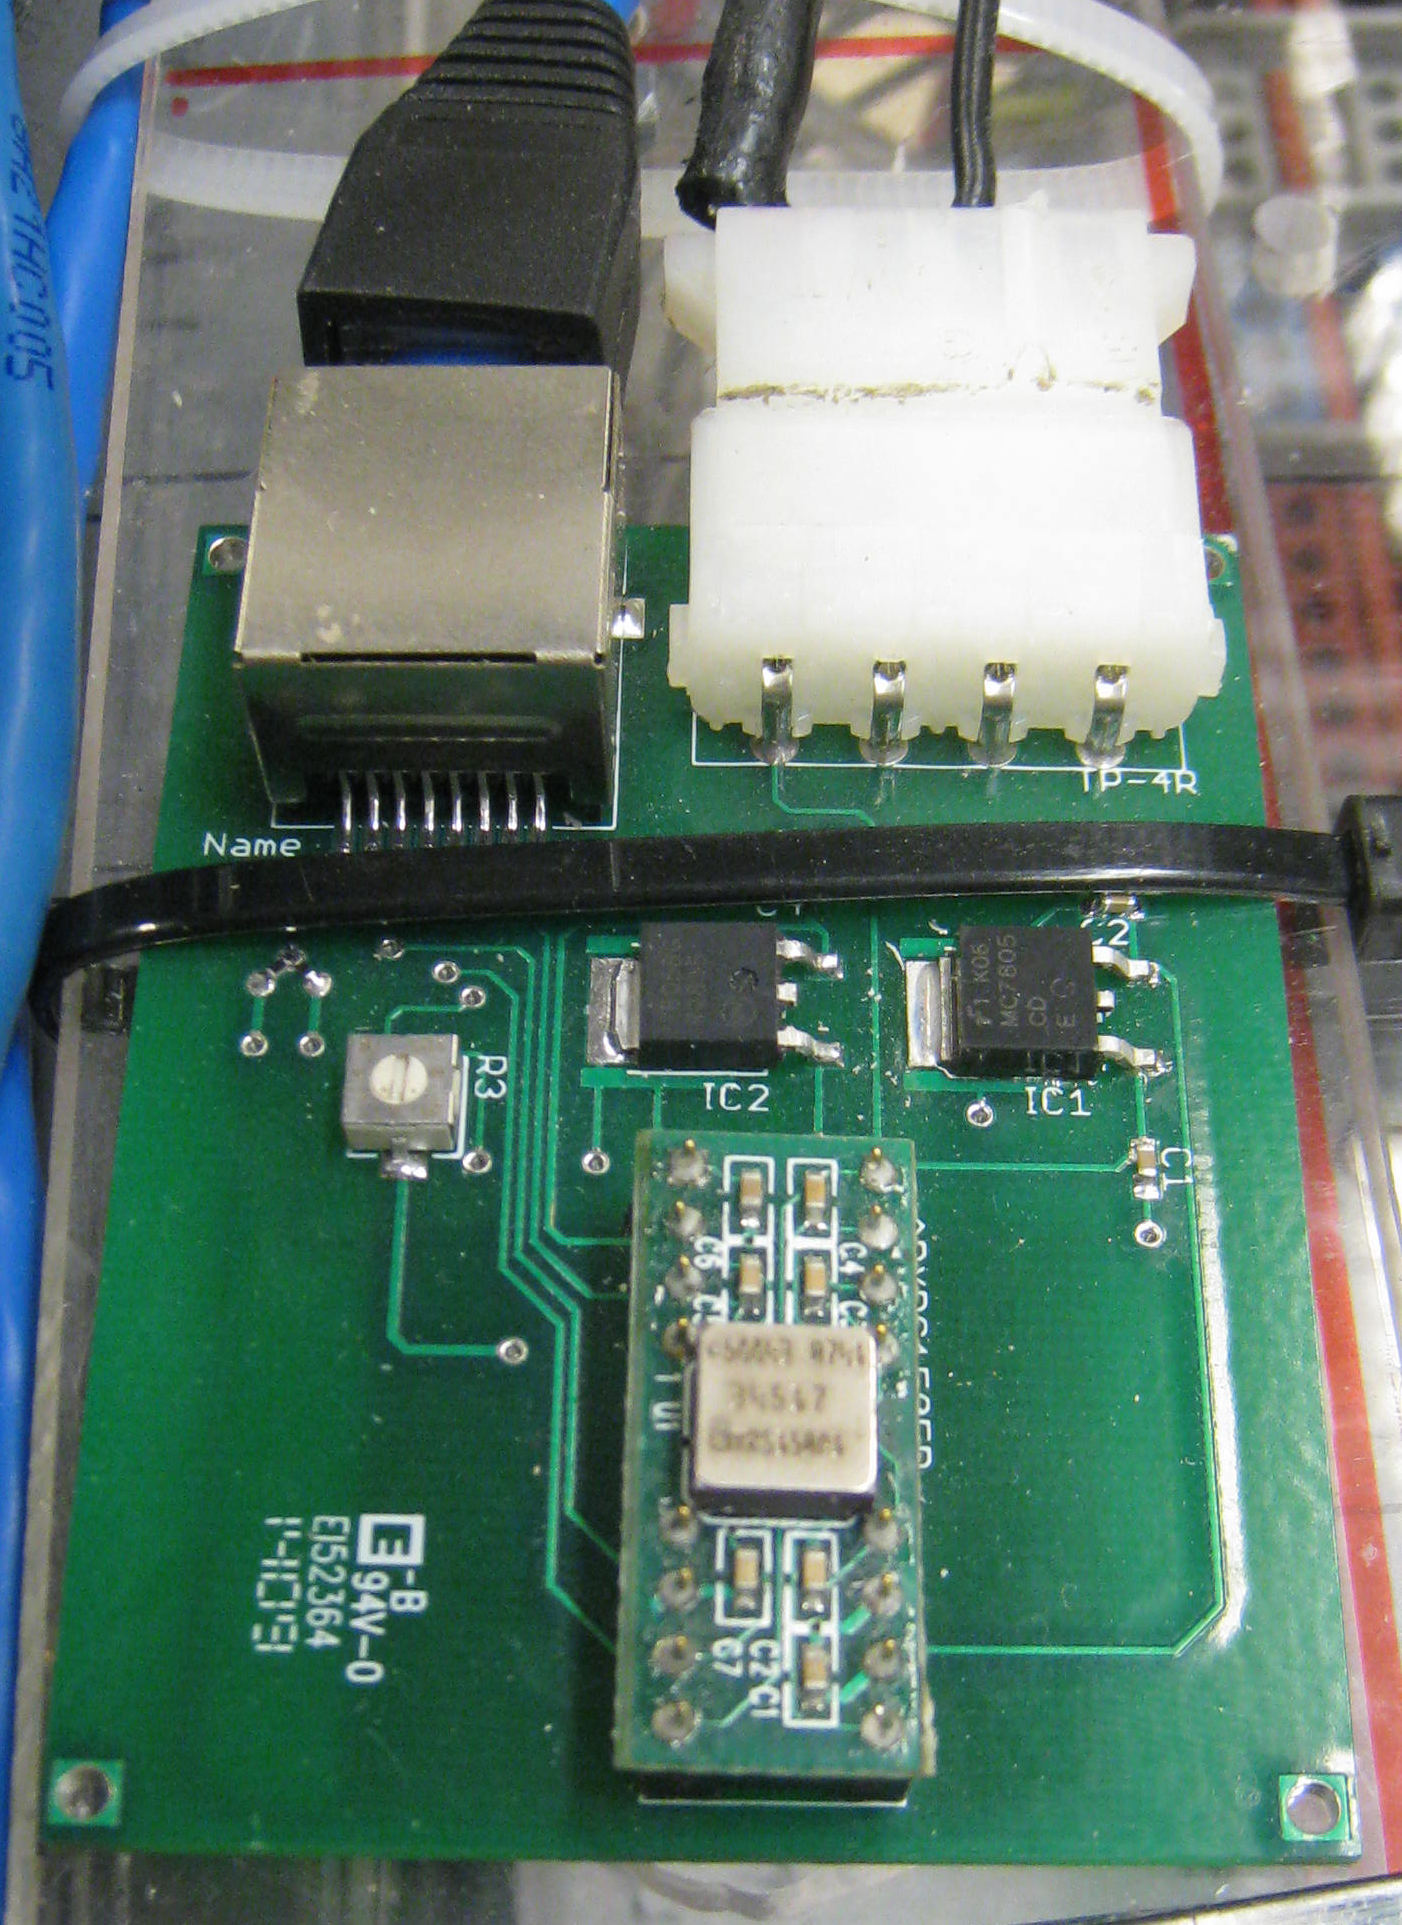
\includegraphics[width=0.5\textwidth]{images/yaw_rate_sensor}
\caption{Analog Devices ADXRS150 Gyro as mounted on HARLIE \label{fig:yaw_rate_sensor}}
\end{figure}

The third sensor on HARLIE used for indoor localization is the SICK LIDAR (see \autoref{fig:sick_lms291}).

\begin{figure}
\centering
\subfloat[SICK LMS291]{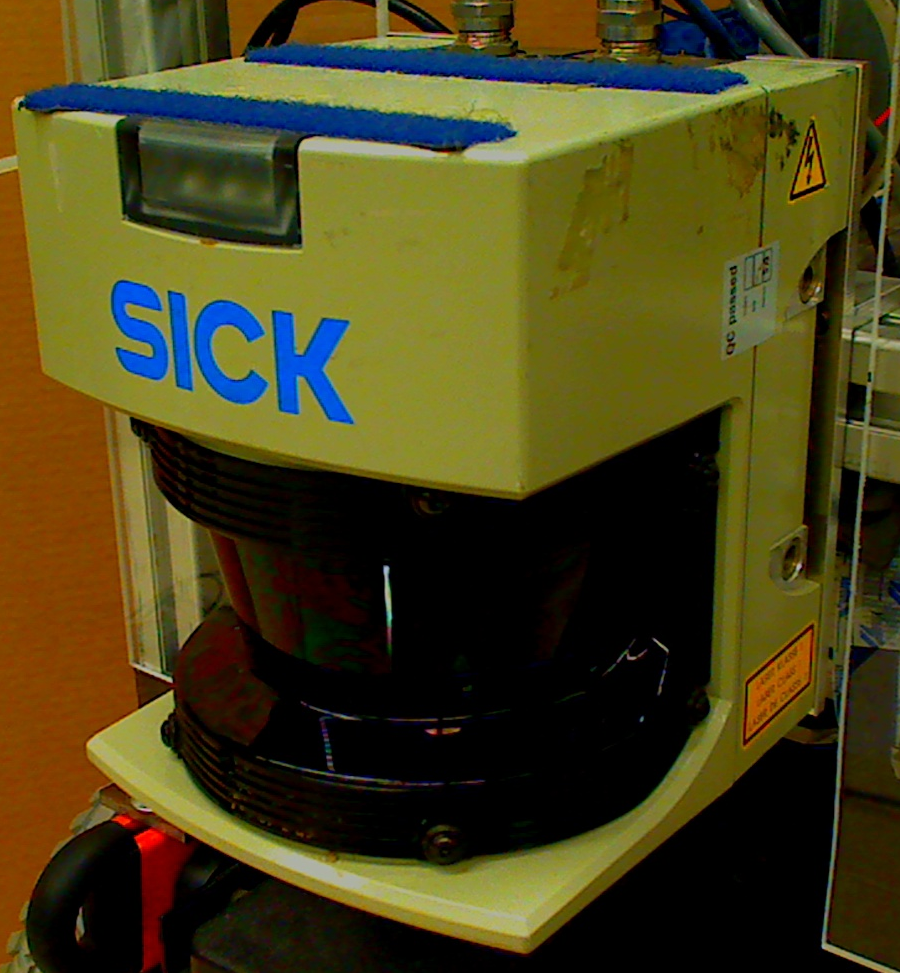
\includegraphics[width=0.4\textwidth]{images/sick_lms291}\label{fig:sick_lms291}}
\hfill
\subfloat[Sample LIDAR Scan \autocite{WikipediaSICKScan}]{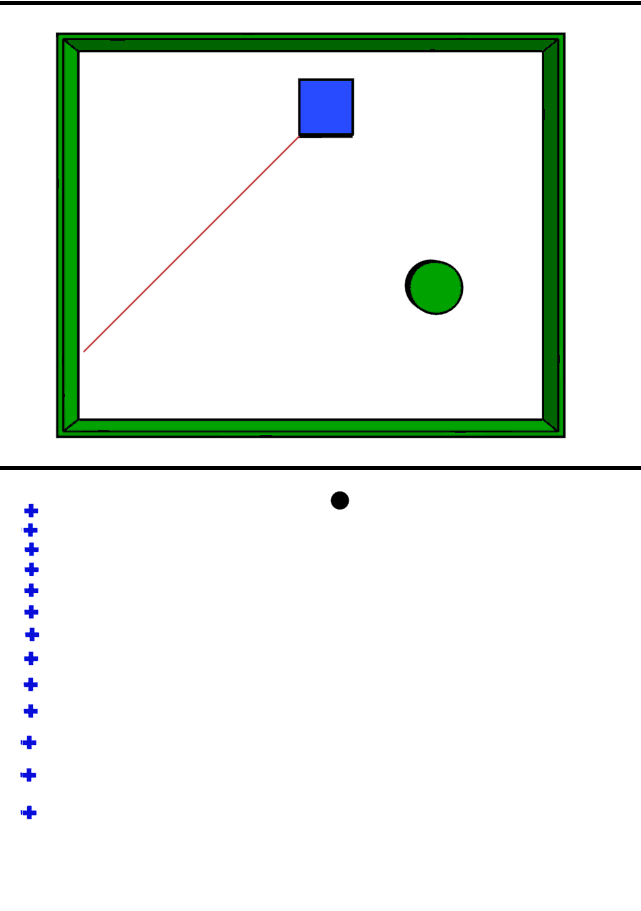
\includegraphics[width=0.4\textwidth]{images/sample_scan}\label{fig:sample_sick_scan}}
\caption{SICK LIDAR \& Sample LIDAR Scan}
\label{fig:sick_and_sample_scan}
\end{figure}

\subsection{Simulation}\label{subsec:simulation_setup}

Gazebo simulation
